\documentclass[10pt,letterpaper]{article}

\usepackage[spanish]{babel}
\usepackage{fontspec}
\setmainfont{Arial}
\setsansfont{Arial}
\setmonofont{Consolas}
\usepackage[letterpaper,left=1.2in,right=1.2in,top=0.88in,bottom=0.52in,headheight=44pt,headsep=9pt,footskip=24pt]{geometry}
\usepackage{graphicx}
\usepackage{fancyhdr}
\usepackage{enumitem}
\usepackage{xcolor}
\usepackage{listings}
\usepackage{microtype}
\usepackage{array}

\definecolor{codigofondo}{RGB}{218,218,218}
\definecolor{lineaazul}{RGB}{157,184,218}
\definecolor{textoazul}{RGB}{45,91,147}

\pagestyle{fancy}
\fancyhf{}
\fancyhead[L]{
\includegraphics[height=1.1cm]{figuras/sello-upt.jpg}}
\fancyhead[R]{\textcolor{textoazul}{\footnotesize Escuela Profesional de Ingeniería de Sistemas}}
\fancyfoot[L]{\textcolor{textoazul}{\footnotesize Mag. Alberto Johnatan Flor Rodríguez}}
\fancyfoot[C]{\textcolor{textoazul}{\footnotesize - \thepage -}}
\renewcommand{\headrulewidth}{0.35pt}
\renewcommand{\footrulewidth}{0.35pt}
\makeatletter
\renewcommand{\headrule}{\hbox to\headwidth{\color{lineaazul}\leaders\hrule height \headrulewidth\hfill}}
\renewcommand{\footrule}{\hbox to\headwidth{\color{lineaazul}\leaders\hrule height \footrulewidth\hfill}}
\makeatother

\setlength{\parindent}{0pt}
\setlength{\parskip}{0.48em}
\linespread{1.08}
\setlength{\emergencystretch}{1em}
\setlist[itemize]{leftmargin=1.5em,itemsep=0.1em,topsep=0.25em,parsep=0.05em}
\setlist[enumerate]{leftmargin=1.8em,itemsep=0.1em,topsep=0.25em,parsep=0.05em}
\renewcommand{\familydefault}{\sfdefault}


\lstset{
  basicstyle=\ttfamily\fontsize{8.5}{9.7}\selectfont,
  backgroundcolor=\color{codigofondo},
  frame=single,
  rulecolor=\color{black!55},
  framerule=0.35pt,
  framesep=4pt,
  breaklines=true,
  breakatwhitespace=false,
  columns=fullflexible,
  keepspaces=true,
  showstringspaces=false,
  xleftmargin=0pt,
  xrightmargin=0pt,
  aboveskip=0.35em,
  belowskip=0.4em,
  tabsize=2,
  upquote=true
}


\newcommand{\tocline}[2]{
\noindent #1
\nobreak\dotfill
\nobreak #2\par}

\newcommand{\tocsub}[2]{
\noindent\hspace*{1.05em}#1
\nobreak\dotfill
\nobreak #2\par}

\newcommand{\ruledheading}[1]{\par\vspace{0.2em}
\noindent\textbf{#1}\par
\noindent\rule{\linewidth}{0.45pt}\par}

\newcommand{\blankline}{
\noindent\rule{\linewidth}{0.35pt}\par\vspace{0.30in}}

\begin{document}

% Página 1: portada
\thispagestyle{empty}
\begin{center}
\vspace*{0.75in}
{\large\bfseries UNIVERSIDAD PRIVADA DE TACNA\par}
{
ormalsize\bfseries FACULTAD DE INGENIERÍA\par}
{
ormalsize\bfseries ESCUELA DE INGENIERÍA DE SISTEMAS\par}
\vspace{0.26in}

\includegraphics[width=1.48in]{figuras/logo-epis.png}\par
\vspace{0.13in}
{\LARGE\bfseries Guía Práctica de Laboratorio\par}
\vspace{0.48in}
{\Large\bfseries “Implementación de Room Database en Kotlin”\par}
\vspace{0.50in}
{\small\bfseries Que se presenta para el curso:\par}
{\small\bfseries “SOLUCIONES MOVILES I”\par}
\vspace{0.63in}
{\small\bfseries Docente:\par}
{\small\bfseries Mag. Alberto Johnatan Flor Rodríguez\par}
\vfill
{\small\bfseries TACNA – PERÚ\par}
{\small 2026\par}
\end{center}

% Página 2: índice

\newpage
\setcounter{page}{2}
\begin{center}
\vspace*{0.18in}
{\large\bfseries Índice General}
\end{center}
\vspace{0.18in}
\small
\tocline{Introducción}{3}
\tocline{Guía de Laboratorio Nº 06 “Implementación de Room Database en Kotlin”}{4}
\tocline{1. Información sobre el evento práctico}{4}
\tocsub{1.1. Título del evento práctico}{4}
\tocsub{1.2. Objetivos}{4}
\tocsub{1.3. Tiempo de duración (horas)}{4}
\tocsub{1.4. Resultados de Aprendizaje (RA)}{4}
\tocsub{1.5. Recursos (Equipos, materiales, programas y otros)}{4}
\tocline{2. Procedimiento o Metodología}{4}
\tocline{3. Conclusiones (especifique por lo menos 3)}{13}
\tocline{4. Cuestionario}{13}
\tocline{5. Referencias Bibliográficas}{14}

% Página 3: introducción

\newpage
\begin{center}
\vspace*{0.62in}
{\large\bfseries Introducción\par}
\end{center}
\vspace{0.13in}
En el desarrollo de aplicaciones Android modernas, la persistencia de datos es un pilar fundamental para ofrecer una experiencia de usuario fluida, permitiendo que la información se mantenga disponible incluso sin conexión a internet o tras cerrar la aplicación. Room Database se presenta como una capa de abstracción sobre SQLite que facilita el acceso fluido a la base de datos, aprovechando toda la potencia de SQLite mientras proporciona una verificación de consultas en tiempo de compilación.

Este laboratorio práctico se centra en la arquitectura de persistencia recomendada por Google. Los estudiantes aprenderán a estructurar una base de datos local utilizando los tres componentes clave de Room:

\begin{enumerate}
  \item Entity: Que representa las tablas de la base de datos.
  \item DAO (Data Access Object): Que define los métodos para acceder a los datos.
  \item Database: Que sirve como el punto de acceso principal para la conexión.
\end{enumerate}

Además, se integrará el uso de Corrutinas de Kotlin y el componente ViewModel para asegurar que las operaciones de entrada/salida (I/O) se realicen de forma asíncrona, manteniendo la interfaz de usuario reactiva y libre de bloqueos..

% Página 4: información y comienzo del procedimiento

\newpage
\begin{center}
\vspace*{0.12in}
{\bfseries Guía de Laboratorio Nº 06 “Implementación de Room Database en Kotlin”\par}
\end{center}
\vspace{0.08in}
\ruledheading{1. Información sobre el evento práctico}

\textbf{1.1. \quad Título del evento práctico}

\hspace*{1.55em}Implementación de Room Database en Kotlin.

\textbf{1.2. \quad Objetivos}
\begin{itemize}
  \item Implementar Room como medio de almacenamiento interno de información.
  \item Integrar Workers con Corrutinas mediante el uso de Dispatchers.IO para optimizar el uso de hilos.
\end{itemize}

\textbf{1.3. \quad Tiempo de duración (horas)}

\hspace*{1.55em}2 Horas

\textbf{1.4. \quad Resultados de Aprendizaje (RA)}
\begin{itemize}
  \item El estudiante gestiona tareas de larga duración fuera del hilo principal, garantizando la persistencia de los procesos incluso si la aplicación se cierra.
  \item Aplica el principio de separación de responsabilidades delegando la lógica de trabajo pesado a Workers especializados.
\end{itemize}

\textbf{1.5. \quad Recursos (Equipos, materiales, programas y otros)}
\begin{itemize}
  \item Computadora con acceso a internet.
  \item Android Studio (Versión más reciente).
  \item Dispositivo físico Android o creación de un Android Virtual Device (AVD).
\end{itemize}

\ruledheading{2. Procedimiento o Metodología}
\textbf{Inicio de la aplicación}

Creamos un nuevo proyecto en Adroid Studio con una empty activity:

% Página 5: asistentes de creación del proyecto

\newpage
\begin{center}
\vspace*{0.02in}
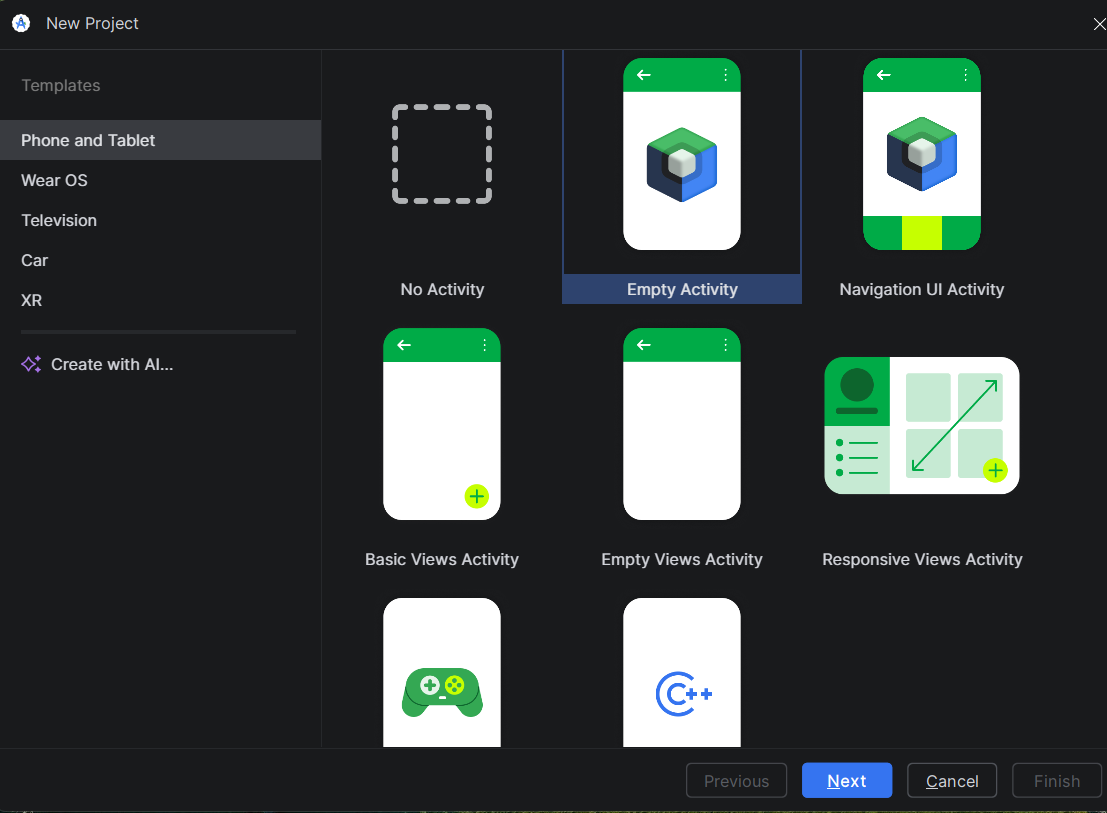
\includegraphics[width=5.55in]{figuras/android-studio-proyecto.png}\par
\vspace{0.10in}
\end{center}
Colocamos de nombre roomDatabase:
\begin{center}
\vspace{0.03in}
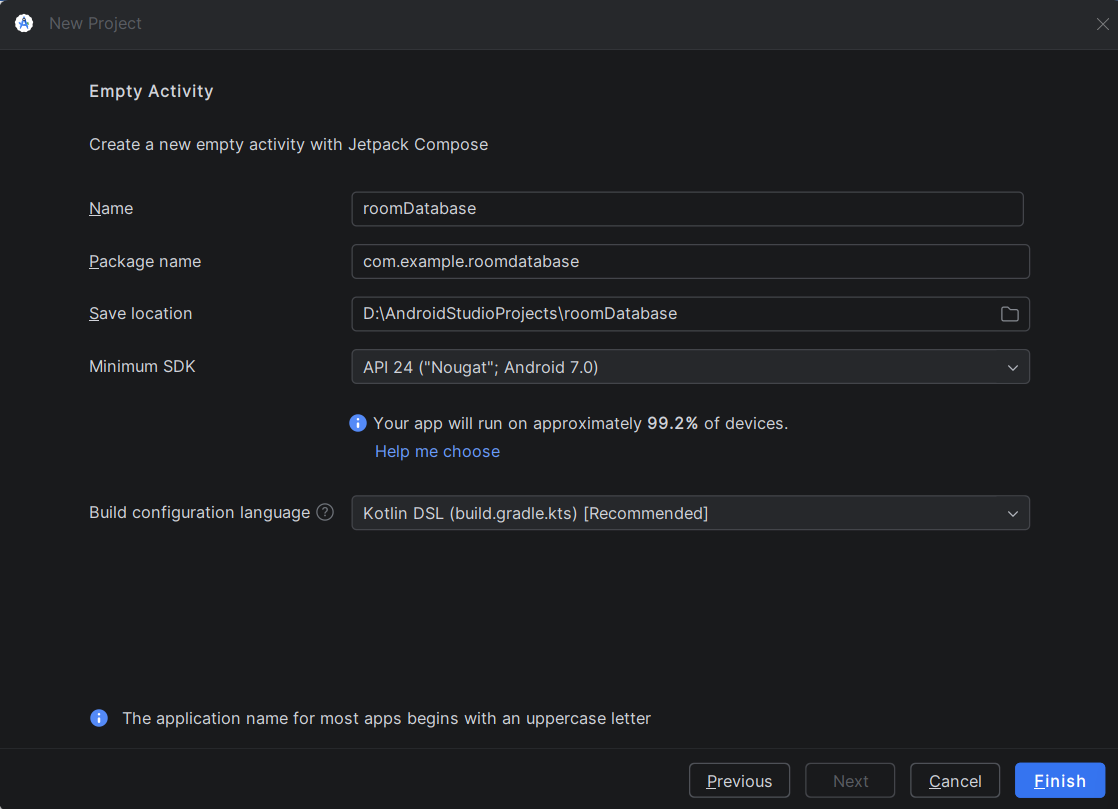
\includegraphics[width=5.48in]{figuras/android-studio-configuracion.png}
\end{center}

% Página 6: distribución propuesta

\newpage
\textbf{Clases a trabajar y disposición en la aplicación:}

Se propone trabajar la siguiente distribución de clases para cubrir la sencilla lógica de un mantenimiento de tablas a traves de las bibliotecas Room:

\begin{lstlisting}
@startuml

package "UI Layer" {
  class MainActivity {
    - viewModel: MainViewModel
    + onCreate()
  }
  class MainViewModel {
    + insertUser()
    + insertUserList()
    + updateUser()
    + deleteUser()
    + getAllUsers()
  }
}
package "Application" {
  class RoomApplication {
    {static} + db: AppDatabase
    + onCreate()
  }
}
package "Data Layer (Room)" {
  abstract class AppDatabase {
    + {abstract} userDao(): UserDao
  }

  interface UserDao <<interface>> {
     + insertUser(user: UserEntity): Long
     + insertUserList(people: List<UserEntity>): List<Long>
     + updateUser(user: UserEntity): Int
     + deleteUser(user: UserEntity): Int
     + getAll(): List<UserEntity>
     + getAllById(userIds: IntArray): List<UserEntity>
  }

  class UserEntity <<data>> {
    + userId: Int
    + nombres: String?
    + apellidos: String?
  }
}
' Relationships
MainActivity --> MainViewModel : usa
MainViewModel --> RoomApplication : accede db
RoomApplication o-- AppDatabase : mantiene instanciado
AppDatabase ..> UserDao : provee
UserDao ..> UserEntity : opera con
@enduml
\end{lstlisting}

% Página 7: diagrama UML

\newpage
\begin{center}
\vspace*{0.03in}
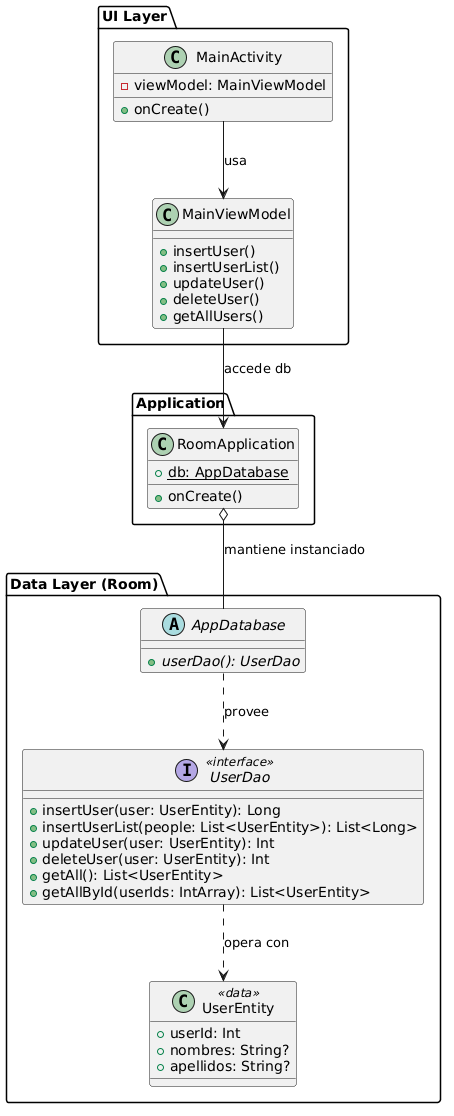
\includegraphics[height=8.65in,keepaspectratio]{figuras/diagrama-clases.png}
\end{center}

% Página 8: configuración de dependencias

\newpage
Iniciamos con la configuración de los scripts de la aplicación, de modo tal que podamos sincronizar el uso de las bibliotecas de Android:

Para esto modificamos el fichero “libs.versions.toml” agregando las versiones del compilador de la siguiente forma:

\begin{lstlisting}
[versions]
…
kotlin = "2.3.21"
composeBom = "2026.04.01"
kotlinskp = "2.3.4"
…

[plugins]
android-application = { id = "com.android.application", version.ref = "agp" }
kotlin-compose = { id = "org.jetbrains.kotlin.plugin.compose", version.ref = "kotlin" }
kotlinksp = {id= "com.google.devtools.ksp", version.ref = "kotlinskp"}
\end{lstlisting}

Luego modificamos el fichero “build.gradle.kts” del proyecto de la siguiente forma:

\begin{lstlisting}
plugins {
  …
  alias(libs.plugins.kotlinksp) apply false
}
\end{lstlisting}

Finalmente modificamos el fichero “build.gradle.kts” de la aplicación:

\begin{lstlisting}
plugins {
  …
  alias(libs.plugins.kotlinksp)
}

…
dependencies {
  val room_version = "2.8.4"

    implementation("androidx.room:room-runtime:$room_version")

    ksp("androidx.room:room-compiler:$room_version")
    annotationProcessor("androidx.room:room-compiler:$room_version")
    implementation("androidx.room:room-ktx:$room_version")
…
}
\end{lstlisting}

Ahora vamos a generar los paquetes necesarios para poder comprender el funcionamiento de las clases del proyecto, los cuales son: application, data\{dao,database,entity\}, ui y viewmodel.

% Página 9: estructura de paquetes y entidad

\newpage
\begin{center}
\vspace*{0.02in}
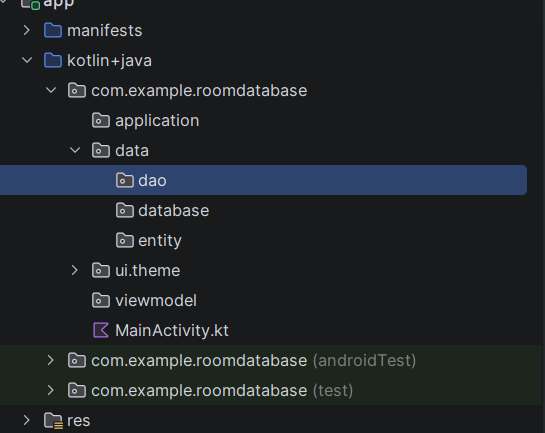
\includegraphics[width=4.45in]{figuras/estructura-paquetes.png}
\end{center}

Ahora procedemos a crear la data class UserEntity que será la representación de la tabla “users”:

\begin{lstlisting}
package com.example.roomdatabase.data.entity

import androidx.room.ColumnInfo
import androidx.room.Entity
import androidx.room.PrimaryKey

@Entity(tableName = "users")
data class UserEntity(
  @PrimaryKey(autoGenerate = true) val userId: Int = 0,
  @ColumnInfo(name = "first_name") val nombres: String?,
  @ColumnInfo(name = "last_name") val apellidos: String?
)
\end{lstlisting}

Luego procedemos a definir la interface que permitirá trabajar con la entidad, esto a través de la interface UserDao en el paquete dao:

\begin{lstlisting}
package com.example.roomdatabase.data.dao

import androidx.room.Dao
import androidx.room.Delete
import androidx.room.Insert
import androidx.room.OnConflictStrategy
\end{lstlisting}

% Página 10: DAO, database y comienzo de Application

\newpage
\begin{lstlisting}
import androidx.room.Query
import androidx.room.Update
import com.example.roomdatabase.data.entity.UserEntity

@Dao
interface UserDao {
   @Insert(onConflict = OnConflictStrategy.ABORT)
   suspend fun insertUser(user: UserEntity):Long
   @Insert(onConflict = OnConflictStrategy.ABORT)
   suspend fun insertUserList(people: List<UserEntity>): List<Long>
   @Update
   suspend fun updateUser(user: UserEntity): Int
   @Delete
   suspend fun deleteUser(user: UserEntity): Int
   @Query("SELECT * FROM users")
   suspend fun getAll(): List<UserEntity>
   @Query("SELECT * FROM users WHERE userId IN (:userIds)")
   suspend fun getAllById(userIds: IntArray): List<UserEntity>?
}
\end{lstlisting}

Para orquestar con la base de datos, procederemos a definirla a través de la clase abstracta, la cual llamaremos AppDatabase, la cual heredará los métodos de RoomDatabase:

\begin{lstlisting}
package com.example.roomdatabase.data.database

import androidx.room.Database
import androidx.room.RoomDatabase
import com.example.roomdatabase.data.dao.UserDao
import com.example.roomdatabase.data.entity.UserEntity

@Database(entities = [UserEntity::class], version = 1)
abstract class AppDatabase : RoomDatabase() {
  abstract fun userDao(): UserDao
}
\end{lstlisting}

Para poder tener una instancia única de la base de datos, vamos a crear una clase que herede de Application con companion object, que tendrá dicho propósito:

\begin{lstlisting}
package com.example.roomdatabase.application

import android.app.Application
import androidx.room.Room
import com.example.roomdatabase.data.database.AppDatabase

class RoomApplication: Application (){
  companion object {
    lateinit var db: AppDatabase
  }

  override fun onCreate() {
    super.onCreate()
    db = Room.databaseBuilder(
\end{lstlisting}

% Página 11: cierre de Application, Manifest y ViewModel

\newpage
\begin{lstlisting}
        applicationContext,
        AppDatabase::class.java,
        "database-users").build()
  }
}
\end{lstlisting}

Para completar la llamada a esta última clase, vamos a modificar el fichero AndroidManifest.xml, indicando el nombre de la aplicación con la clase:

\begin{lstlisting}
<?xml version="1.0" encoding="utf-8"?>
<manifest xmlns:android="http://schemas.android.com/apk/res/android"
  xmlns:tools="http://schemas.android.com/tools">

    <application
      android:name=".application.RoomApplication"
      android:allowBackup="true"
      android:dataExtractionRules="@xml/data_extraction_rules"
      android:fullBackupContent="@xml/backup_rules"
      android:icon="@mipmap/ic_launcher"
      android:label="@string/app_name"
      android:roundIcon="@mipmap/ic_launcher_round"
      android:supportsRtl="true"
      android:theme="@style/Theme.RoomDatabase">
      <activity
        android:name=".MainActivity"
        android:exported="true"
        android:label="@string/app_name"
        android:theme="@style/Theme.RoomDatabase">
        <intent-filter>
           <action android:name="android.intent.action.MAIN" />

           <category android:name="android.intent.category.LAUNCHER" />
        </intent-filter>
      </activity>
    </application>

</manifest>
\end{lstlisting}

Ahora se debe crear el ViewModel, que nos servirá para la ejecución de las instrucciones que gestionan la base de datos:

\begin{lstlisting}
package com.example.roomdatabase.viewmodel

import androidx.lifecycle.ViewModel
import androidx.lifecycle.viewModelScope
import com.example.roomdatabase.application.RoomApplication
import com.example.roomdatabase.data.entity.UserEntity
import kotlinx.coroutines.Dispatchers
import kotlinx.coroutines.launch

class MainViewModel: ViewModel() {
  fun insertUser() {
    val userEntity = UserEntity(nombres = "Juan", apellidos = "Perez")
\end{lstlisting}

% Página 12: ViewModel y operaciones iniciales

\newpage
\begin{lstlisting}
    viewModelScope.launch(Dispatchers.IO){
       RoomApplication.db.userDao().insertUser(userEntity)
    }
  }
  fun insertUserList() {
    val users = listOf(
       UserEntity(nombres = "Juan", apellidos = "Perez"),
       UserEntity(nombres = "Maria", apellidos = "Lopez"),
       UserEntity(nombres = "Pedro", apellidos = "Gonzalez"),
       UserEntity(nombres = "Ana", apellidos = "Martinez"),
       UserEntity(nombres = "Luis", apellidos = "Garcia")
    )
    viewModelScope.launch(Dispatchers.IO){
       RoomApplication.db.userDao().insertUserList(users)
    }
  }
}
\end{lstlisting}

Ahora para probar nuestro ViewModel, vamos a agregarlo en el fichero MainActivity.kt:

\begin{lstlisting}
class MainActivity : ComponentActivity() {

    private val viewModel:MainViewModel by viewModels()
    override fun onCreate(savedInstanceState: Bundle?) {
      super.onCreate(savedInstanceState)

      viewModel.insertUser()
      viewModel.insertUserList()

      enableEdgeToEdge()
   …
\end{lstlisting}

Para completar la solución, modificamos el fichero MainViewModel, otorgando la funcionalidad de los métodos que faltan:

\begin{lstlisting}
fun updateUser(){
     val userEntity = UserEntity(userId = 1, nombres = "Jorge", apellidos = "Perez")
     viewModelScope.launch(Dispatchers.IO){
        RoomApplication.db.userDao().updateUser(userEntity)
        println("DEBUG: Usuario actualizado correctamente")
     }
  }
  fun deleteUser() {
     val userEntity = UserEntity(userId = 4,"","")
     viewModelScope.launch(Dispatchers.IO) {
        RoomApplication.db.userDao().deleteUser(userEntity)
     }
  }
  fun getAllUsers(){
     viewModelScope.launch(Dispatchers.IO){
        val users = RoomApplication.db.userDao().getAll()
        users.forEach { user ->
\end{lstlisting}

% Página 13: final, conclusiones, cuestionario y enunciado

\newpage
\begin{lstlisting}
             println("DEBUG: ${user.userId} - ${user.nombres} - ${user.apellidos}")
        }
     }
  }
\end{lstlisting}

Finalmente, agregamos las instrucciones al MainActivity:

\begin{lstlisting}
private val viewModel:MainViewModel by viewModels()
override fun onCreate(savedInstanceState: Bundle?) {
  super.onCreate(savedInstanceState)

     viewModel.updateUser()
     viewModel.deleteUser()
     viewModel.getAllUsers()
\end{lstlisting}

\ruledheading{3. Conclusiones (especifique por lo menos 3)}
\blankline\blankline\blankline\blankline\blankline\blankline\blankline
\ruledheading{4. Cuestionario}

\begin{enumerate}
  \item ¿Cuál es la función principal de la anotación @Dao y qué ventaja ofrece sobre el\\uso directo de \mbox{SQLiteOpenHelper}?
  \item En la clase UserEntity, se utilizó @PrimaryKey(autoGenerate = true). Explique qué sucede si se intenta insertar un objeto con el userId inicializado en 0.
  \item ¿Por qué es necesario ejecutar las funciones del DAO dentro de un bloque\\viewModelScope.launch(Dispatchers.IO)? ¿Qué sucedería si se ejecutan en el hilo principal?
  \item Explique el propósito de crear una clase que hereda de Application (como RoomApplication) para inicializar la base de datos.
  \item ¿Qué función cumple el motor KSP (Kotlin Symbol Processing) configurado en los archivos build.gradle.kts en relación con Room?
\end{enumerate}

\textbf{Enunciado}

Una vez implementada la estructura básica de UserEntity y su respectivo mantenimiento, se requiere escalar la aplicación para que sea funcional para un usuario final, añadiendo validaciones y una visualización de datos más robusta.

% Página 14: ampliación solicitada y referencias originales

\newpage
\begin{enumerate}[label=\arabic*.]
  \item \textbf{Modificación de la Entidad:}
    \begin{itemize}
      \item Agregue un nuevo campo a la clase UserEntity llamado email de tipo String (debe permitir valores nulos).
      \item Actualice la versión de la base de datos en AppDatabase a la versión 2 y configure una política de migración destructiva básica (\texttt{.fallbackToDestructiveMigration()}) en el Room.databaseBuilder.
    \end{itemize}

  \item \textbf{Implementación de Búsqueda:}
    \begin{itemize}
      \item Añada un nuevo método en UserDao que permita buscar usuarios por su apellido (last\_name) utilizando la cláusula LIKE de SQL.
      \item Implemente la función correspondiente en el MainViewModel.
    \end{itemize}

  \item \textbf{Integración de UI (Interfaz de Usuario):}
    \begin{itemize}
      \item En el MainActivity, diseñe una interfaz sencilla (usando Jetpack Compose) que contenga:
        \begin{itemize}[label=$\circ$]
          \item Dos campos de texto (Nombre y Apellido).
          \item Un botón para "Guardar Usuario".
          \item Un componente de lista (LazyColumn o RecyclerView) que muestre los usuarios guardados actualmente en la base de datos.
        \end{itemize}
    \end{itemize}

  \item \textbf{Lógica de Negocio:}
    \begin{itemize}
      \item Asegúrese de que la lista de usuarios se actualice automáticamente en la pantalla cada vez que se inserte o elimine un registro.
    \end{itemize}
\end{enumerate}

\ruledheading{5. Referencias Bibliográficas}
\begin{itemize}
  \item Android Developers (2026). Ciclo de vida de la actividad. Recuperado de la documentación oficial de Android.
  \item Android Developers (2026). Guía de WorkManager: Programación de tareas asíncronas. Recuperado de la documentación oficial de Android Jetpack.
  \item Kotlin Foundation (2025). Coroutines Guide: Dispatchers and Context.
  \item Android Developers (2026). Common Architecture Patterns: MVVM with Repository and Jetpack Work.
\end{itemize}

\end{document}

